\documentclass[12pt]{article}
\usepackage[osf]{mathpazo}
\usepackage{ms}
\usepackage{natbib}
\usepackage{lineno}
\usepackage{graphicx}
\usepackage{caption}
\modulolinenumbers[5]
\linenumbers

\title{How much of the world is woody?}
\author{
Richard G. FitzJohn$^{*,1}$\\ Matthew W. Pennell$^{*,2,3}$,\\ Amy E. Zanne$^{4}$,\\ William K. Cornwell$^{5}$
}
\date{}
\affiliation{\noindent
$^*$ These authors contributed equally}
% RGF: Why have a different running head to the main title?  They have
% the same number of characters!
\runninghead{The proportion of woody species}

\begin{document}
\mstitlepage
\parindent=1.5em
\addtolength{\parskip}{.3em}

\begin{abstract}
% RGF: Not sure if I'll get to it, but the first part of the abstract
% is too long.  It's nice though, and could be rolled into the main
% text.

%WKC: needs to be 200 words
%
Through large databases and synthetic research, a picture of global biodiversity is beginning to emerge, but especially with regard to global functional diversity, basic questions remain.   The woody/herbaceous divide is perhaps the most fundamental axis of functional diversity among plants.  We sought to address a very basic question with regard to global plant functional diversity: what proportion of the world's species are woody? Surprisingly, this question has never been comprehensively addressed.  We combined a plant functional trait database to date with two gap--filling approaches.  We estimate the proportion ``woodiness'' among the world's vascular plants to be between 45\% and 48\%.  We sought to determine whether a consensus answer to our question existed among botanists---even if not formally documented in the peer-reviewed literature. To investigate this, we coupled our analysis with a survey in which we posed our question to the broader community of botanists and other biologists.  We found that no expert consensus existed and that, on average, researchers underestimated the proportion of the world's flora that was woody. The results of our survey highlight that global datasets can show patterns at odds with conventional wisdom.  Global plant functional diversity is much woodier than we thought.  
\end{abstract}

\section{Introduction}


% RGF: This seems like a weaker opening sentence than we'd like.
% Perhaps ignore the distinction between wood and pseudo wood for now
% an introduce this later.
%
% Was thinking about something along the lines of "It is trivial to
% observe that some species are woody and others are not, yet..."
The distinction between a woody and non-woody growth-form of plants is
probably the most profound contrast among terrestrial plants and
ecosystems: the difference between a forest and a grassland is the
presence or absence of wood. The recognition of the fundamental
importance of this divide dates back at least to \textit{Enquiry into
  Plants} by Theophrastus of Eresus (371 -- 287 BC), a student of
Plato and Aristolte, who began his investigation into plant form and
function by classifying the hundreds of plants in his garden into
woody and herbaceous categories \citep{theophrastus1916enquiry}. Functionally, not all wood is ``true wood'' (i.e., secondary thickness of the xylem).  Palms are
``functionally'' woody, having a very long-lived above-ground stem and long generation time.  Even Theophrastus both recognized the fundamentally importance of the  distinction between woody and herbaceous plants, and that this distinction is in some difficult to make.   

% An alternative here would be to structure this like (I've just
% arbitrarily jotted things down here).  Also may depend on a
% definition of "true" woodiness in the preceeding paragraph.  
The last two thousand years of research into wood since Theophrastus
classified his garden have uncovered its origin in the early Devonian
\citep[$\sim$~400 mya;][]{gerrienne2011simple}; that prevalence of
woodiness varies with climate \citep{judd1994}; that wood has been
lost many times in diverse groups (both extant and extinction); that
many different ways of pseudo-woody growth habit have appeared across
groups that have lost true woodiness (or diverged before true
woodiness evolved).  We know about its mechanical properties and
developmental pathways, its patterns of decomposition and their
effects on ecosystem function \citep{Cornwellwood}.  Woody and
herbaceous species have different rates of morphological evolution and
may diversify at different rates \citep{SmithDonoghue}.
%
However, surprisingly we have no idea about what proportion of species
are actually woody.


%
% Also see here
% http://iphylo.blogspot.ca/2011/10/how-many-species-are-there-and-why-do.html
% for some nice discussion of the differences between the Mora and
% Costello papers (do look into the comments at the bottom).

With the rise of bioinformatics, the similar biodiversity question of
``how many species are there on earth'' can be approached with a variety of different methods
\citep{may1988many,erwin1991many, stork1993many, joppa2010,
  costello2011, mora2011plos}.  These statistical estimates are
improved , narrowing in most recently on a number around 8.7 million
species with around 300,000 of those plants \citep{mora2011plos}, although other approaches have come to different estimates \citep{costello2011}.
% 
% --------------------------------------------------------------------
% RGF: I'm really not convinced about what this 1/2 para and the
% following paragraph add.  First, I don't think that a phylogenetic
% approach and a functional approach are alternatives (you could look
% at functional traits in a phylogenetic context, for example).  I'm
% not sure that investigating species' strategies depends on there
% being 8.7 million species -- is that a large number or a small
% number?  What is the contrast?  If there were only 4000 species it
% would be interesting (that's probably about as many species as there
% are in NZ, for example).
%
% The second paragraph seems to be trying to justify one method over
% another when I don't feel that they are necessarily alternatives.
%
% You had a really nice link that these two paragraph fell between, so
% I've stitched them together that way.
% --------------------------------------------------------------------
% 
% My preference would probably be to drop these, and I've commented
% them out accordingly.  If there are points in here that I've missed
% then we should work out more clearly what they are and what they add
% and put them in the right place.  Perhaps discussion?  
% It is also becoming clear that in a world with 8.7 million species,
% the clear next step toward a systematic understanding of that
% diversity is a system to understand the structure of that
% diversity. There are two complementary approaches to address this
% problem: a phylogenetic approach, in which diversity is structured
% according to shared ancestry and a functional approach, following
% Theophrastus \citep[more recently in the tradition
% of][]{grime1979plant, weiher2009challenging, westoby2002plant}, that
% essentially asks how many different ways do species make their living
% and how many species are in each category?
% 
% Global taxonomic and phylogenetic efforts, although still not perfect,
% are much closer to being globally complete compared to the functional
% approach.  There has been a great deal of progress is assembling both
% taxonomies and phylogenies for the huge numbers of species including
% plants \citep[e.g.][]{smith2011understanding}. But despite their
% importance for understanding ecosystem services and making
% conservation decisions, we are only just beginning to assemble
% analogous databases that describe the functional characteristics of
% those species \citep{Kattge2011TRY}. The fact that phylogenetic
% efforts are a good deal more advanced than functional ones is
% surprising given the 2000-year history of the functional approach and
% the 250-year history of the taxonomic approach.
% 
% Interestingly, because taxonomic efforts are ahead of functional
% efforts, they can be used in combination with functional database to
% formulate estimates of the global structure of functional
% biodiversity.
Here, we aim to use similar tools to re-ask Theophrastus' 2000 year
old question at the global scale: how many of the world's plant
species are woody?
% 
We felt that such a basic question would be essentially known.  But
upon consulting the literature, we discovered that surprisingly little
had been written on this topic. We then posed the question to several
botanical experts and received a tremendous variety of answers in
response suggesting that this fundamental aspect of plant functional
diversity was surprisingly poorly understood. 

Here we undertake the first attempt, to our knowledge, to try and
quantify the proportion of woodiness across the world's flora. We also
took the unconventional approach of coupling our analysis of the data
with a survey in which we asked our question to the broader community
of botanists and other biologists. The motivation for this was to
determine whether a consensus answer did exist---even if not
formalized in the literature---and if so, whether it was consistent
with the data.

% I think this is a strong end to the intro, and the paragraph that
% followed it is better suited in the methods, results and/or discussion.

% Though the experimental design of our survey was not ideal (e.g. we
% relied on voluntary response) and certainly biased in terms of who
% responded, we were none-the-less able to demonstrate the novelty of
% this project. Not only was there a huge variance in responses but
% the mean and median estimates from the survey were far from our
% those estimate obtained from analyzing available data. This evidence
% suggests that researchers' intuitions regarding the proportion of
% woody plants may be severely misinformed. [THE END OF THE
% INTRODUCTION IS WEAK]

\section{Methods and Materials}

\subsection{Dataset}

We used a recently assembled database with growth--form data for
49,064 species, which is the largest database assembled to date.  
% Which number do we want to use here?  The number of rows in the raw
% data when ignoring issues such as "variable" and synonymy?
%   path.forest <- readLines("~/.forest_path")
%   dat <- read.csv(file.path(path.forest, "export/speciesTraitData.csv"), stringsAsFactors=FALSE)
%   sum(!is.na(dat$woodiness))
% which gives 49,064 species.
% 
% Alternatively, we could use the fully processed number 
%   sum(dat.g$K)
% which gives 37,488 species.
% 
% I've gone with the former for now.
%
%WKC: Matt and I agree with this choice
%
In this dataset, we defined woodiness as the persistence of a
perennial above--ground stem, which includes palms and tree ferns as
woody---species that are excluded by strict anatomical definitions of
``wood''.  
% This is a bit confusing as this "intermediate" is different to
% non-strict woody, but the sentence follows along.
There are a number of species which are intermediate in form \citep{beaulieuHiddenRates}; in this dataset 633 species (1.3\%) were coded
as variable.  For the formal analysis we excluded these species.
Because the effort to organize plant taxonomy, especially synonymy, is
on-going, there was uncertainty regarding the status of many of these
plant names.  We matched this database with the accepted names from
the plant list (www.theplantlist.org) leading to 37,488 records with documented
taxonomy---15,657 herbs and 21,831 woody species.  This included records from all plant orders currently accepted by APG-III (ref).  
% sum(dat.g$K) # known species
% sum(dat.g$H) # herbs
% sum(dat.g$W) # 

% RGF: Describe how we sorted out fern synonomy and got the accepted
% number of species?  Or was that just the allies?  Or just the higher
% order taxonomy.

%WKC:  compare family sampling to total number of families? Somehow show the dataset is comprehensive?

\subsection{Estimating the fraction of species that are woody}

We cannot simply use the fraction of species within our trait database
(21,831 / 37,488 = 58\%) as these records represent a biased sample of
vascular plants.
% sum(dat.g$W) # woody
% sum(dat.g$K) # known
% sum(dat.g$W) / sum(dat.g$K) # fraction
For example, most Orchidaceae are probably herbaceous; we have only
two records of woodiness among the 1,574 species for which we have
data.
% i.orc <- dat.g$family == "Orchidaceae"
% sum(dat.g$K[i.orc]) # known Orchidaceae
% sum(dat.g$W[i.orc]) # woody Orchidaceae
However, the fraction of Orchidaceae with known data (1,574 / 27,104 =
6\%)
% sum(dat.g$K[i.orc]) # known Orchidaceae
% sum(dat.g$N[i.orc]) # number of Orchidaceae
% sum(dat.g$K[i.orc]) / sum(dat.g$N[i.orc]) # knowledge rate of Orchidaceae
is much lower than the overall rate of knowledge over all vascular
plants (36,238 / 274,141 = 13\%), which will downwardly bias the
global estimate of woodiness.
% sum(dat.g$K) # known vascular
% sum(dat.g$N) # total vascular
% sum(dat.g$K) / sum(dat.g$N) # knowlege rate for all vascular plants
%
Conversely, systematic under-sampling of tropical species, believed to
be more woody than temperate species \citep{Molesheihgt}, would bias
the global woodiness estimate downwards.

To impute the state (i.e., woody or herbaceous) of species with
unknown states, we used a simple Monte Carlo method to sample species
states.  We either assumed that (a) the observed species were drawn
with no replacement from a pool of species while making no assumption
about the distribution of states within the pool (``weak prior'') or
(b) that the observed species were drawn from a very large pool of
species with a fraction of woody species equal to the fraction of
woodiness among known species within the genus (``strong prior'').
%
For genera with no known states, we sampled a woodiness fraction from
the empirical distribution of woodiness fractions for other genera
within the same order.
%
We repeated the above sampling approach 1,000 times and report means
and confidence intervals over this distribution.
%
This procedure is described in detail in the appendix to this paper.

\subsection{Survey}

% RGF: I've tried to motivate the survey a bit more.  It's still
% pretty sketchy, but I think it puts the emphasis in a better place.
We were surprised to find little consensus within our working group,
so proceeded to investigate if a general consensus among
biologists existed.
% 
% RGF: I've put folk knowledge here, but it's the wrong term and needs
% replacing.
Along similar lines, \citet{joppa2010} found that botanical experts generally predicted the
total number of species within plant groups, and we were interested in
whether there was similar anecdotal knowledge for the relative prevalence of
this key trait.
%
We created an English-language survey asking for an estimate of the
fraction of species that are woody.  We also asked respondents to
indicate their level of familiarity with plants, level of formal
training, and the country in which they received their training (see
supplementary material \ref{fig:survey-text} for details).
% Were other lists used?  I've assumed that it is and changed the
% language.  I'd be inclined to drop mention of the departmental
% lists, as that's a similar level to just bugging people in the
% department, which is what I did.
We distributed the survey to the community via several electronic
mailing lists with wide circulation among biologists: \emph{EvolDir},
\emph{ECOLOG}, \emph{r-sig-phylo}, \emph{Taxacom}, \emph{Herbaria}, as
well as local lists. We also posted links on the social-networking platforms \textsc{google+},
\textsc{twitter} and \textsc{facebook} to reach as broad an audience
as we could.
% RGF: can we be specific about the Brazilian mailing lists?
In order to increase representation of survey responses from Latin
America, we translated the survey into Portuguese (thanks to Rafael
Maia) and distributed it to various Brazilian biology
\textsc{facebook} groups and university mailing lists.

% RGF: A logistic transform is different to a logistic regression.
To analyze the survey data, we performed logistic regression, with the percent woodiness as the response variable \citep[for discussion as to why we used logistic regression, see][]{wartonarcsine} and treating the various levels of familiarity and education as ordered factors.


\section{Results and Discussion}

% RGG: The paragraph that was here largely rehashed the first
% paragraph of the paper, and is not needed in such a short paper I
% think (commented below for reference).

% A global picture of biodiversity requires taxonomic, genetic and
% functional components.  In many ways research into function is the
% oldest of these lines of research, but today our functional
% understanding of global biodiversity is not as developed as our
% taxonomic and genetic understanding. Woodiness is a fundamental
% plant trait for many reasons: the presence or absence of wood
% structures the main difference between terrestrial biomes; woody and
% herbaceous species also evolve at different rates
% \citep{SmithDonoghue}; there are also important evolutionary
% interactions with climate (Zanne); and wood itself has crucial
% effects on the global carbon cycle \citep{Cornwellwood}.  The
% question we ask in this paper---how many of the world's plant
% species are woody---is an extremely basic global description of
% global functional diversity.

% The three paragraphs below probably can be spliced together in a
% more convincing order.  The middle paragraph might be a better
% concluding paragraph?

Across all vascular plants, we estimated the fraction woody species to
be between 45\% to 48\%.
% round(100*res.strong$overall, 1)
% round(100*res.weak$overall, 1)
Specifically, using our ``strong prior'' sampling approach we
estimated 45.0\% (95\% CI of 44.7--45.3\%) and with the ``weak prior''
approach we estimated 47.2\% (95\% CI of 46.6--47.8\%).  
% 
The different approaches generate different distributions of the
per-genus fraction of woodiness (Figure
\ref{fig:distribution-genera}~b), with a less strongly bimodal
distribution using the ``weak prior'' approach, as we describe in the
appendix.
%
This difference in the predicted distribution drives the difference in
the estimates of woodiness.  Genera that are primarily herbaceous
(fraction of woody species less than 10\% for genera with at least 10
records) were on average larger than primarily woody genera (more than
90\% woody species), with 202 species rather than 138.
%

Higher--order classifications are at least as much a product of human
pattern matching as any biological pattern.  Genera probably
correspond to the classification differences that humans deem
important \citep{scotland2004significance}, which likely includes woodiness.  
The relative paucity of genera with significant numbers of
both woody and herbaceous species (Figure
\ref{fig:distribution-genera}) reinforces the importance of this
trait.

Because the observed distribution of woodiness fraction among genera
is itself very bimodal, we are inclined to believe that the true
result lies closer to 45\% than to 47\%.  A more sophisticated
hierarchical modeling approach could probably lead to a more precise
answer, but we feel that our values probably span the range of
estimates that such a modeling approach would generate.  
%
Probably a larger problem is that undiscovered species are unlikely to
be random with respect to woodiness.  In principle, rarefaction
analysis could estimate the number of species remaining to be
discovered in different groups, but this is not possible for many
plant clades \citep{costello2011}.
%
In any case, such a simple question as this deserves a simple answer.

% RGF: Given the discussion I had with Amy yesterday, we might want to
% swap out the phylogeny for the one I did for Jeremy's paper.  Or at
% least move to having the bars around the outside.  I can have a look
% at that if you'd like.  Might be nicer than the spots that we
% currently have.  I'm not sure we can realistically get the families
% around the outside of the tree with diversity information though;
% they're about as packed in as we can take it.  However, the tree
% does look really quite ugly and I'd like to see what this looks like
% trimmed down.  Anyone up for looking at how easy it will be to
% anchor orders against one of the time trees and see how it looks
% when pruned that way?

% RGF: Not sure what we could possibly write here that would be
% interesting.  If we're not going to add anything interesting in
% here, then should we simply drop the phylogeny figures?
The distribution of woodiness varies widely among different taxonomic
groups (Figure \ref{fig:phylogeny}).  There are two major clades that
are primarily herbaceous --- the monocots and Monilophyte (ferns).
However, there are many primarily herbaceous clades nested within
woody clades, and vice versa, which makes the combination of taxonomic and functional information crucial for answering this type of question.  The two different approaches (strong versus weak priors) led to similar taxonomic distributions of estimated woodiness (Figure \ref{fig:phylogeny} versus Figure \ref{fig:phylogeny-supp}).  

% RGF: I didn't like how this immediately started with the apology for
% being different.  I've rewritten this quite a bit.  The next
% paragraph starts with "We have a number of admittedly speculative
% hypotheses as to why this may the case", which is also much more
% carefully hedged than necessary.
In contrast with the very small range in our estimate of the number of
woody species in the world, there is strikingly little consensus among
researchers.  We received 293 responses from 31 countries, which
ranged from estimates of 1\% to 90\% with a mean of 31.7\%.  The vast
majority (81\%) of the responses were less than even our smallest
estimate.
% nrow(d.survey)
% range(d.survey$Estimate)
% mean(d.survey$Estimate < 45)
We found little effect of a respondent's degree of training on their
estimate (Figure \ref{fig:survey}).  There was a significant effect of
the respondent's familiarity with plants on the estimates, primarily
driven by people with very little familiarity with plants (the
``What's a Plant?'' category), whose estimates tended to be the lower
(less woody) than the estimates from other categories.
% 
Before carrying out the survey, we had hypothesized that researchers
from tropical regions may perceive the world as woodier than
researchers from more temperate regions due to the latitudinal
gradient in woodiness \citep{Molesheihgt}.  However, in our informal
survey, respondents who trained in tropical countries were no more
accurate in their predictions than their temperate colleagues (results
not shown).
% RGF: Is the code for doing the classification handy anywhere?  The
% country list is rather long.

We conclude with two observations.  
%
First, most people perceive there to be substantially fewer woody
species in the world than there probably are.  This herb-centric
vision of the world may arise from the importance of our (mostly
herbaceous) cultivated crops, or the fact that people---including researchers---likely
spend more time in the garden than in the forest.
%
Second, there is no consensus as to how woody the world is.  We find
it deeply surprising that this most basic aspect of plant natural
history was not generally known.  Global plant functional diversity is
much woodier than we thought.

\bibliographystyle{ecology}
\bibliography{wood.bib}

\begin{figure}[p]
  \centering
  \includegraphics{figs/fraction-by-genus}
  \caption{Distribution of the fraction of woodiness among genera.
    The distribution of the fraction of species that are woody within
    a genus (among genera) is strongly bimodal (panel a -- showing
    genera with at least 10 species only).
    % 
    The two different sampling approaches generate distributions that
    differ in their bimodality (panel b).  When assuming species are
    sampled with replacement from some pool, but having no prior on
    the fraction of woodiness within the pool generates a broad
    distribution with many polymorphic genera (blue bars), while
    sampling with replacement assuming that species are drawn from a
    pool of species that has a fraction of woody species equal to the
    observed fraction of woodiness generates a strongly bimodal
    distribution.}
  \label{fig:distribution-genera}
\end{figure}

\begin{figure}[p]
  \centering
  \includegraphics{figs/fraction-on-phylogeny}
  \caption{Distribution of the fraction of woodiness among families
    (tips) and orders (nodes) on a phylogeny of vascular plants.
    Darker colours have a higher proportion of woody species,
    estimated using the ``strong prior'' (sampling without
    replacement) approach.  Using the ``weak prior'' approach
    generally adjusts(?) estimates fractions towards 50\% (see Figures
    \ref{fig:distribution-genera} and \ref{fig:distribution-raw}).}
\label{fig:phylogeny}
\end{figure}

\begin{figure}[p]
  \centering
  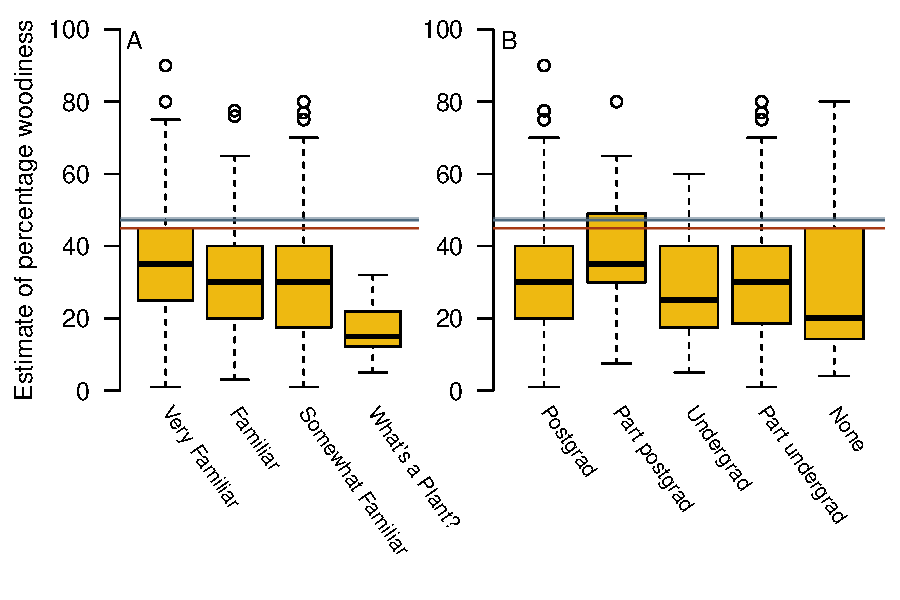
\includegraphics{figs/survey-results}
  \caption{
    Distribution of responses to the survey question ``What percentage
    of the world's vascular plant species are woody?''. Responses are
    broken up by familiarity with plants (panel (a)) and formal
    training in botany or a related discipline (panel (b)). The mean
    and 95\% confidence intervals for our estimates of the proportion
    of woody species from the empirical data are depicted by the horizontal
    shaded rectangles; the upper rectangle corresponds to the ``weak
    prior'' approach and the lower rectangle corresponds to the ``strong
    prior'' approach (see Appendix for details).}
  \label{fig:survey}
\end{figure}

\clearpage
\renewcommand\thefigure{S.\arabic{figure}}
\appendix
\section{Appendix: Sampling proceedure}
\setcounter{figure}{0}    

Here, we describe our algorithm for sampling the states of species
that lack information on woodiness.  We treat each genus separately,
and in all cases know that there are are $n_w$ woody and $n_h$ species
and a total of $N$ species in the genus.
%
For example, the genus \textit{Microcoelia} (Orchidaceae) has 30
species in total, and we know that 17 are herbaceous and none are
known to be woody ($N = 30$, $n_w = 0$, $n_h = 13$).  We do not know
the state of the remaining 17 species, so the true number of woody
species, $N_w$, must lie between 0 and 17.  In general, we can't
assume that these species are all herbaceous, even though both
biological and mathematical intuition suggest that most of them will
be.

We used two different approaches for imputing the values of these
unknown species.  First, we assumed that the known species were
sampled without replacement from a pool of species with $N_w$ woody
and $N_h$ herbaceous species ($N_w + N_h = N$).  The probability that
$x$ of the species are woody ($x = 0, 1, \ldots, N - n_w - n_h$) is
proportional to
\begin{equation}
  \Pr(N_w = x) \propto {n_w + x \choose n_w}
  {N - (n_w + x) \choose n_h}
\end{equation}
For \textit{Microcoelia} this gives a 45\% probability that all
species are herbacious, and a 92\% chance that at most three species
are woody.

This approach probably overestimates the number of woody species in
this case, and in other cases (such as \textit{Actinidia} (Ericaceae)
where all 30 species with known states are woody) will underestimate
the fraction of species that are woody.  We see this as corresponding
to a very weak prior on the shape of the distribution of the fraction
of woody species within a genus.

However, the distribution of woodiness among genera is strongly
bimodal; most genera are either all-woody or all-herbacious (Figure
\ref{fig:distribution-genera}).  Among the 748 genera with at least 10
records, 392 are entirely woody, 248 are entirely herbaceous, and only
50 have between 10\% and 90\% woody species.  As a result, knowing the
state of a handful of species within a genus can give a reasonable
guess at the remaining species.
% tmp <- dat.g$p[dat.g$K >= 10] # genera with 10 records
% sum(tmp == 1) # 100% woody
% sum(tmp == 0) # 100% herbaceous
To model the other extreme of sampling, we used an approach where we
computed the observed fraction of woody species ($p_w = n_w / (n_w +
n_h)$) and sampled the state of the unobserved species using a
binomial distribution, so that the probability that $x$ of the species
are woody is
% RGF: I need to check this when not sleep-deprived/jet lagged. This
% should be an offset binomial distribution.  It may be clearer if we
% define things about numbers of known and unknown species.
\begin{equation}
  \Pr(x = k) = {N - n_w - n_h \choose k - n_w - n_h} 
  p^k (1-p)^{N - n_w - n_h - k}.
\end{equation}

In cases where all known species are woody (or herbaceous) this will
assign all unknown species to be woody (or herbaceous).  In
polymorphic cases this will give similar results method above.  This
approach corresponds to a very strong prior on the shape of the
distribution of woodiness among genera.
% RGF: This is really vague and I will think about it more when I'm
% less braindead.
While neither of these approaches is ``correct'', they probably
span the range of possible outcomes.

For genera where there was no information on woodiness for any
species, we sampled a fraction of species that might be woody from the
empirical distribution of woodiness fractions \textit{among genera}
within the same order.  We did this after imputing the missing species
values within those other genera.  So, if a genus is found in an order
with genera that had woodiness fractions of $\{0, 0, 0.1, 1\}$ we would
have approximately a 50\% chance of sampling a 0\% woodiness fraction
for a genus, with probabilities from 0.1 to 1 being fairly evenly
spread.  Given this woodiness fraction, we then sampled the number of
species that are woody from a binomial distribution with this fraction
and the number of species in the genus as its parameters.

\begin{figure}[p]
  \centering
  \includegraphics{figs/fraction-on-phylogeny-supp}

  \caption{(Supplementary)
    \textit{This is Figure \ref{fig:phylogeny} using the alternative
      sampling approach.}\\
    %
    Distribution of the fraction of woodiness among families
    (tips) and orders (nodes) on a phylogeny of vascular plants.
    Darker colours have a higher proportion of woody species,
    estimated using the ``weak prior'' (sampling with
    replacement) approach.  Using the ``strong prior'' approach
    generally adjusts(?) estimates fractions away 50\% (see Figure
    \ref{fig:phylogeny} and \ref{fig:distribution-genera}).
    }
\label{fig:phylogeny-supp}
\end{figure}

\begin{figure}[p]
  \centering
  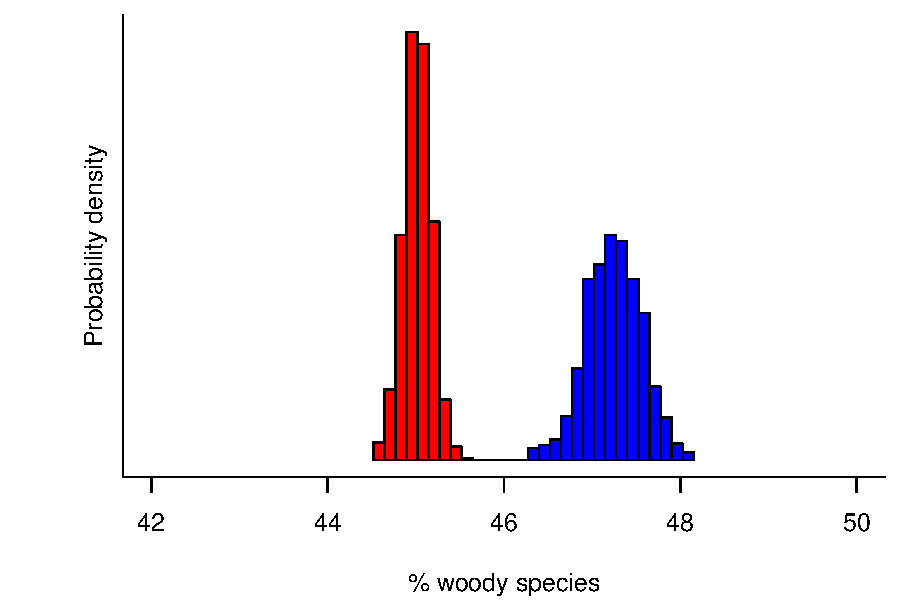
\includegraphics{figs/distribution-raw}  
  \caption{(Supplementary) The posterior probability distribution for
    the proportion of the world's flora that is woody as estimated
    using a) the sampling with replacement (weak prior) and b) without
    replacement (strong prior) method (See Appendix for details).}
  \label{fig:distribution-raw}
\end{figure}

\begin{figure}[p]
  \centering
  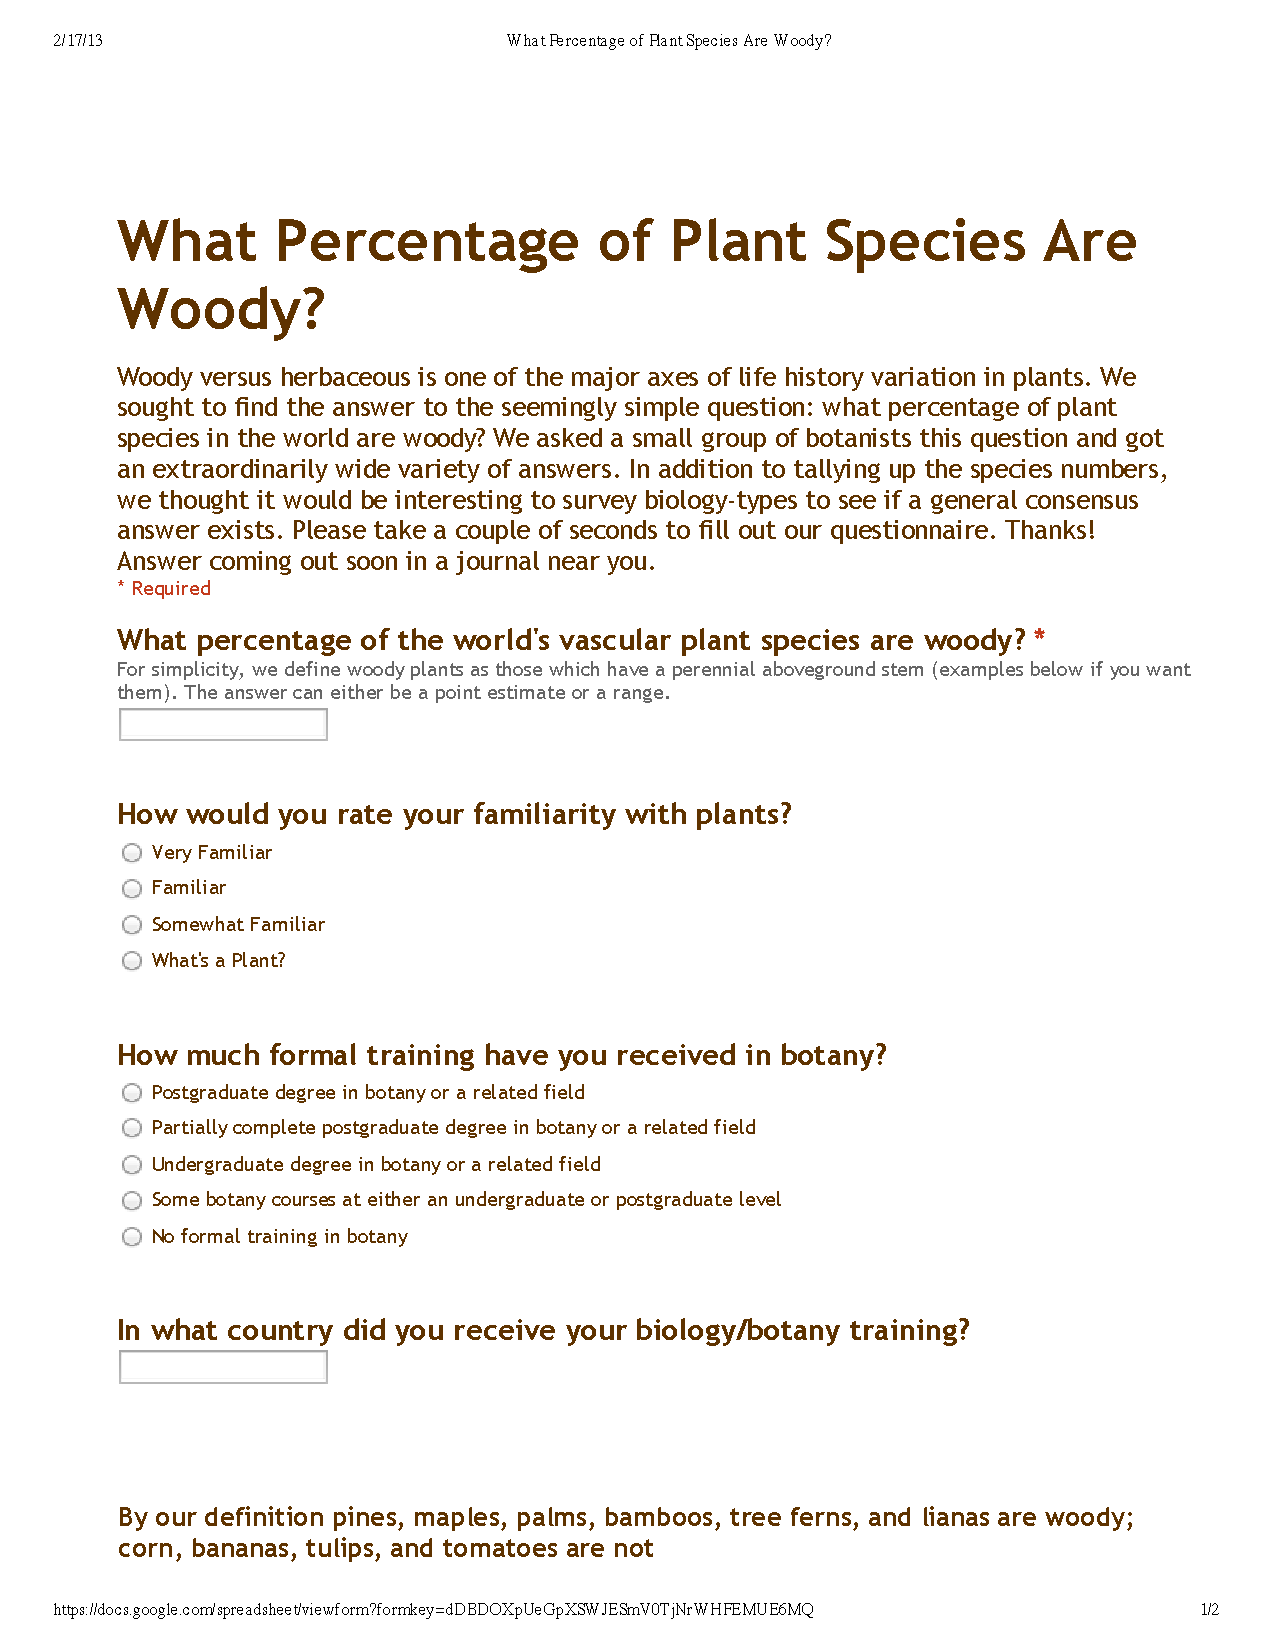
\includegraphics[scale=0.7]{figs/Survey_supplemental}
  \caption{(Supplementary) English-language version of the survey we
    distributed}
  \label{fig:survey-text}
\end{figure}

\begin{figure}[p]
  \centering
  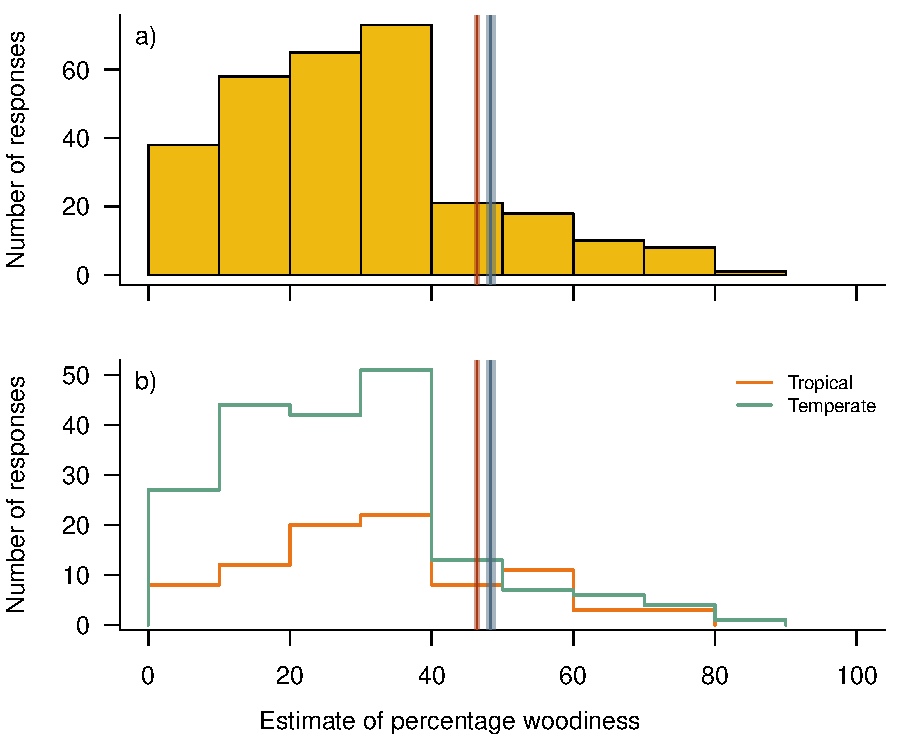
\includegraphics{figs/survey-distribution}
  \caption{(Supplementary) Distribution of all responses to the survey
    question ``What percentage of the world's vascular plant species
    are woody?''.
    %
    The mean and 95\% confidence intervals for our estimates of the
    proportion of woody species from the empirical data are depicted
    by the horizontal shaded rectangles; the blue rectangle corresponds
    to the ``weak prior'' approach and the red rectangle corresponds
    to the ``strong prior'' approach (see Appendix for details).  }

  \label{fig:survey-distribution}
\end{figure}

\end{document}

%%% Local Variables:
%%% mode: latex
%%% TeX-master: t
%%% TeX-PDF-mode: t
%%% End:
